\section{Introduction}
% Delete the text and write your Introduction here:
%------------------------------------



In the field of Machine learning, several methods can be used to solve the same problem. For example, trying to find the local minima using evolutionary algorithms or supervised learning in the form of backpropagation. Both come with advantages and disadvantages depending on if we are after precision or just want to find the local minima fast, but also depending on the nature of our problem.

More specifically interesting is the comparison of the performance of Genetic Algorithms (GA) and Reinforcement Learning (RL) techniques in the context of a game environment. On one hand, in reinforcement learning the agent engages a dynamic and evolving environment by taking actions that affect it to accomplish a specific job. On the other hand, we have evolutionary algorithms that employ evolutionary principles for automated and concurrent problem-solving by drawing inspiration from populations of interacting organisms. Despite their apparent dissimilarities, RL and GA both tackle the same fundamental issue: optimizing a function. This entails maximizing an agent's reward in RL and the fitness function in evolutionary algorithms, respectively, particularly in environments where the parameters may be unknown \cite{drugan2019reinforcement}. 

This paper focuses on comparing Reinforcement learning and Genetic Algorthms by having them balance a cartpole in 500 moves. More specifically it is a problem in nonlinear dynamics where an inverted pendulum is balancing in a cart. The aim or final goal of both RL and GA are to keep it the system balanced until they run out of moves. the environment will be described in more detail under the environment part.  
\begin{figure}[H]
    \centering
    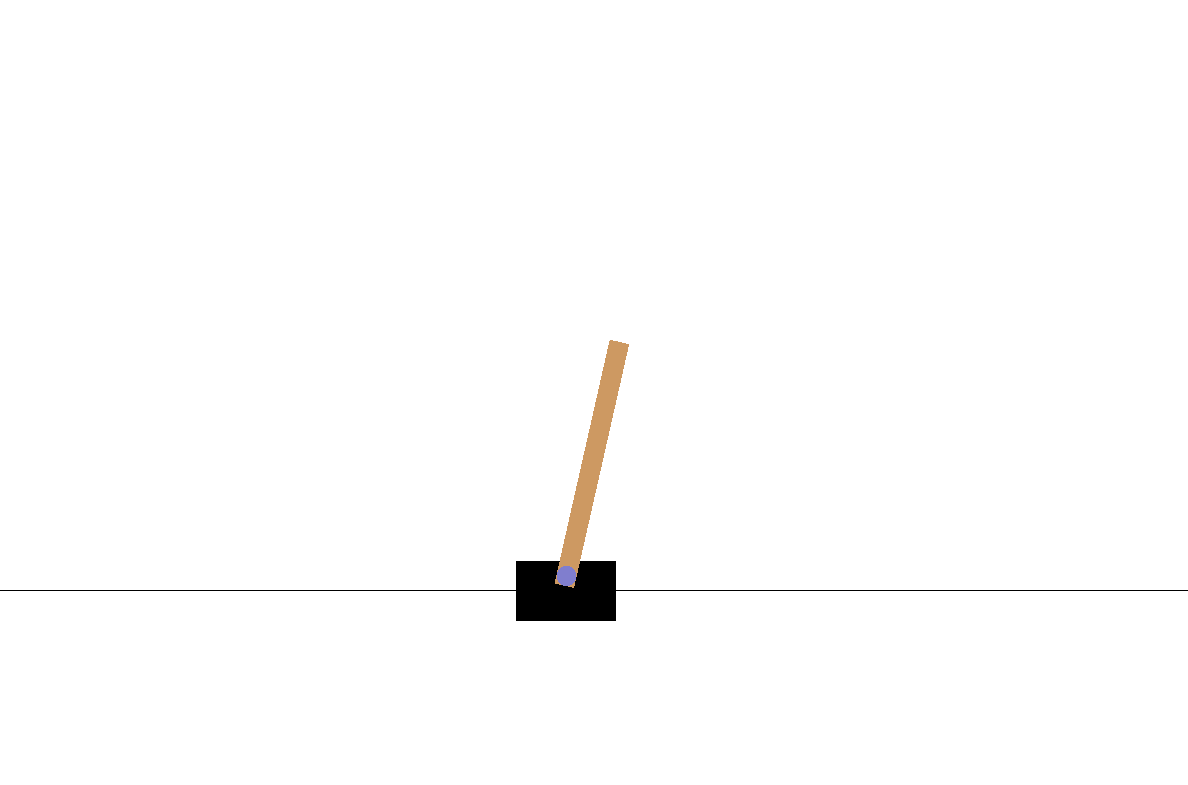
\includegraphics [scale = 0.18]{Images/cartpole.png}
    \caption{the cartpole in 2D graphics}
    \label{figRL}
\end{figure}
Other related research on this topic includes for \cite{drugan2019reinforcement} which focuses on a comprehensive overview of recent trends in the field rather than comparisons of subclasses of algorithms or particular aspects of RL and GA. Several works focus on combining these two methods for machine learning by either using GA to train RL or vice versa such as \cite{eiben2007reinforcement} where the authors try to use Reinforcement learning to tune the parameters of GA.  Papers such as  \cite{khadka2018evolutionary} explore the opposite combination of training RL using GA . It is important to mention that the implementation of the reinforcement learning algorithm that is used is based on the work of \textit{JackFurby} \cite{JackFurbyCartPole}. 



